\section{Conclusion}
\label{sec:conclusion}
\paragraph{}
\par Now, the graphs and values obtained in Section~\ref{sec:analysis} and Section~\ref{sec:simulation} will be presented side by side and compared.
\par The tables and graphs corresponding to Theorical Analysis, through Octave, will be presented on the left, while the Simulation ones made with Ngspice will appear on the right.
\par Firstly, the values of Ripple and Average voltages of both the envelope detector and the voltage regulator can be seen in the following table.

\begin{table}[H]
	\begin{minipage}{.5\linewidth}
		\centering
		\begin{tabular}{|c|c|}
		\hline
		\input{../mat/RipAvg.tex}
		\end{tabular}
		\caption{Ripple and Average Voltages for Envelope and Regulator in Theoretical Analysis}
		\label{table1a}
	\end{minipage}
	\begin{minipage}{.5\linewidth}
		\centering
		\begin{tabular}{|c|c|}
		\hline
		\input{../sim/sim_tab.tex}
	\end{tabular}
 		\caption{Ripple and Average Voltages for Envelope and Regulator in Simulation}
		\label{table1b}
	\end{minipage} 
\end{table}

\par As can be observed, there is some slight inaccuracy between what was obtained theoretically and through simulation, which probably ocurred due to the natural oscilation in the software used (NGSpice). This can explained by the fact that, in oppostition to what happened in previous assignments, there is one component, the diode, which is non-linear meaning there is no linear correlation between current and voltage. The exponential function used in the equations is most likely the cause of said oscilations.
\par That said, it is still an accurate enough result to consider the envelope the detector valid, as the output voltage was, successfully, around 12V.

\par The Merit, calculated through the formula \ref{Merit_Formula} was obtained by both softwares:

\begin{table}[H]
	\begin{minipage}{.5\linewidth}
		\centering
		\begin{tabular}{|c|c|}
		\hline
		\input{../mat/MeritTable.tex}
		\end{tabular}
		\caption{Merit calculated in Theoretical Analysis}
		\label{table1a}
	\end{minipage}
	\begin{minipage}{.5\linewidth}
		\centering
		\begin{tabular}{|c|c|}
		\hline
		\input{../sim/merit_tab.tex}
		\end{tabular}
 		\caption{Merit calculated in Simulation}
		\label{table1b}
	\end{minipage} 
\end{table}

\par As for the voltage values, the Merit values also came with a slight inaccuracy. The Merit value is low, but the group couldn't make it higher, however the main objective of the assignment was achieved.

\par Now let's take a look at the plots done for the output of the Envelope Detector and the Voltage circuits obtained in Theorical Analysis and in Simulation. Also, the comparison between the graphs of $v_o - 12$ (output of AC component plus DC deviation) obtained with Octave and NgSpice.

\begin{figure}[H]
    \includegraphics[width=0.495\linewidth]{all_vout.eps}
    \hfill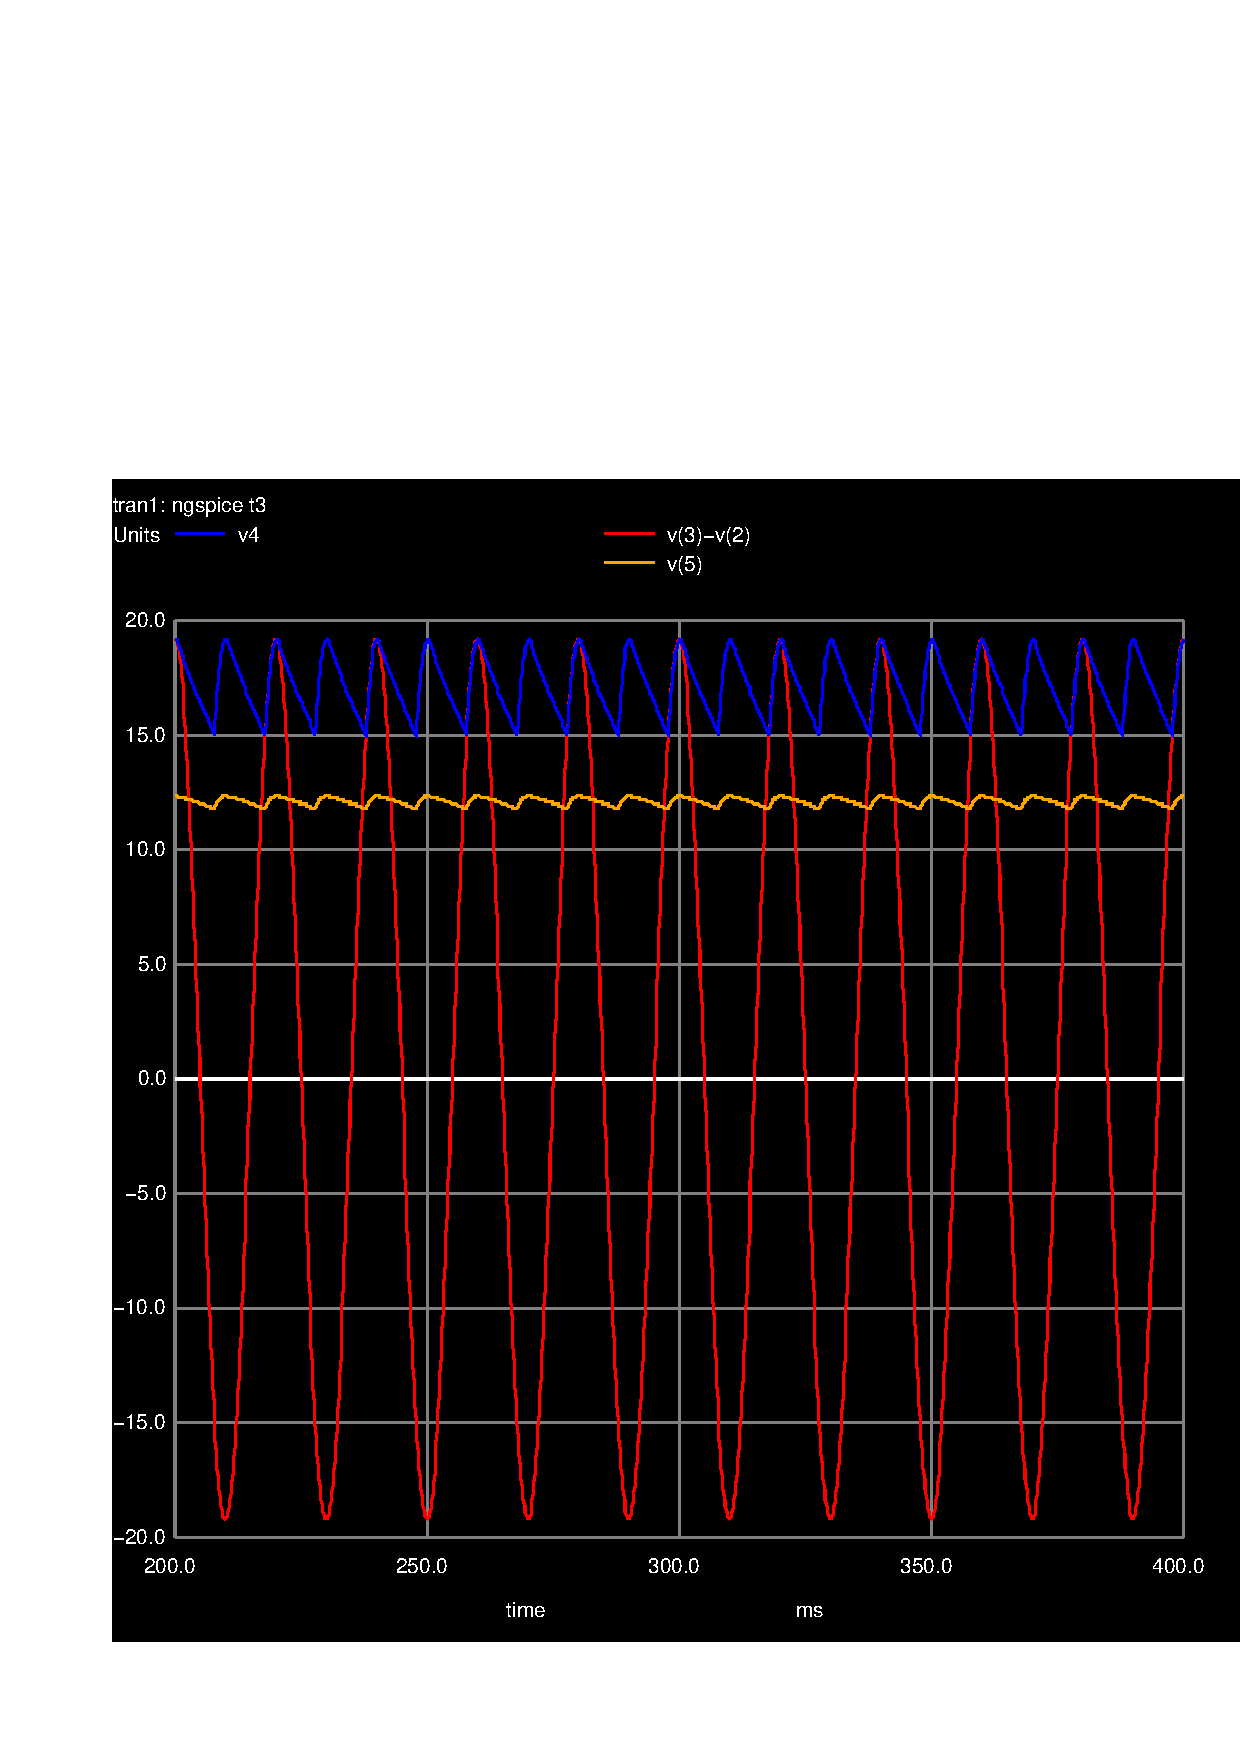
\includegraphics[width=0.4\linewidth]{../sim/comp.pdf}
    \centering
    \caption{Voltage of the rectifier, Voltage of Envelope Detector and Voltage Regulator (Analysis left vs Simulation right)}
    \label{mag}
\end{figure}

\begin{figure}[H]
    \includegraphics[width=0.495\linewidth]{deviation.eps}
    \hfill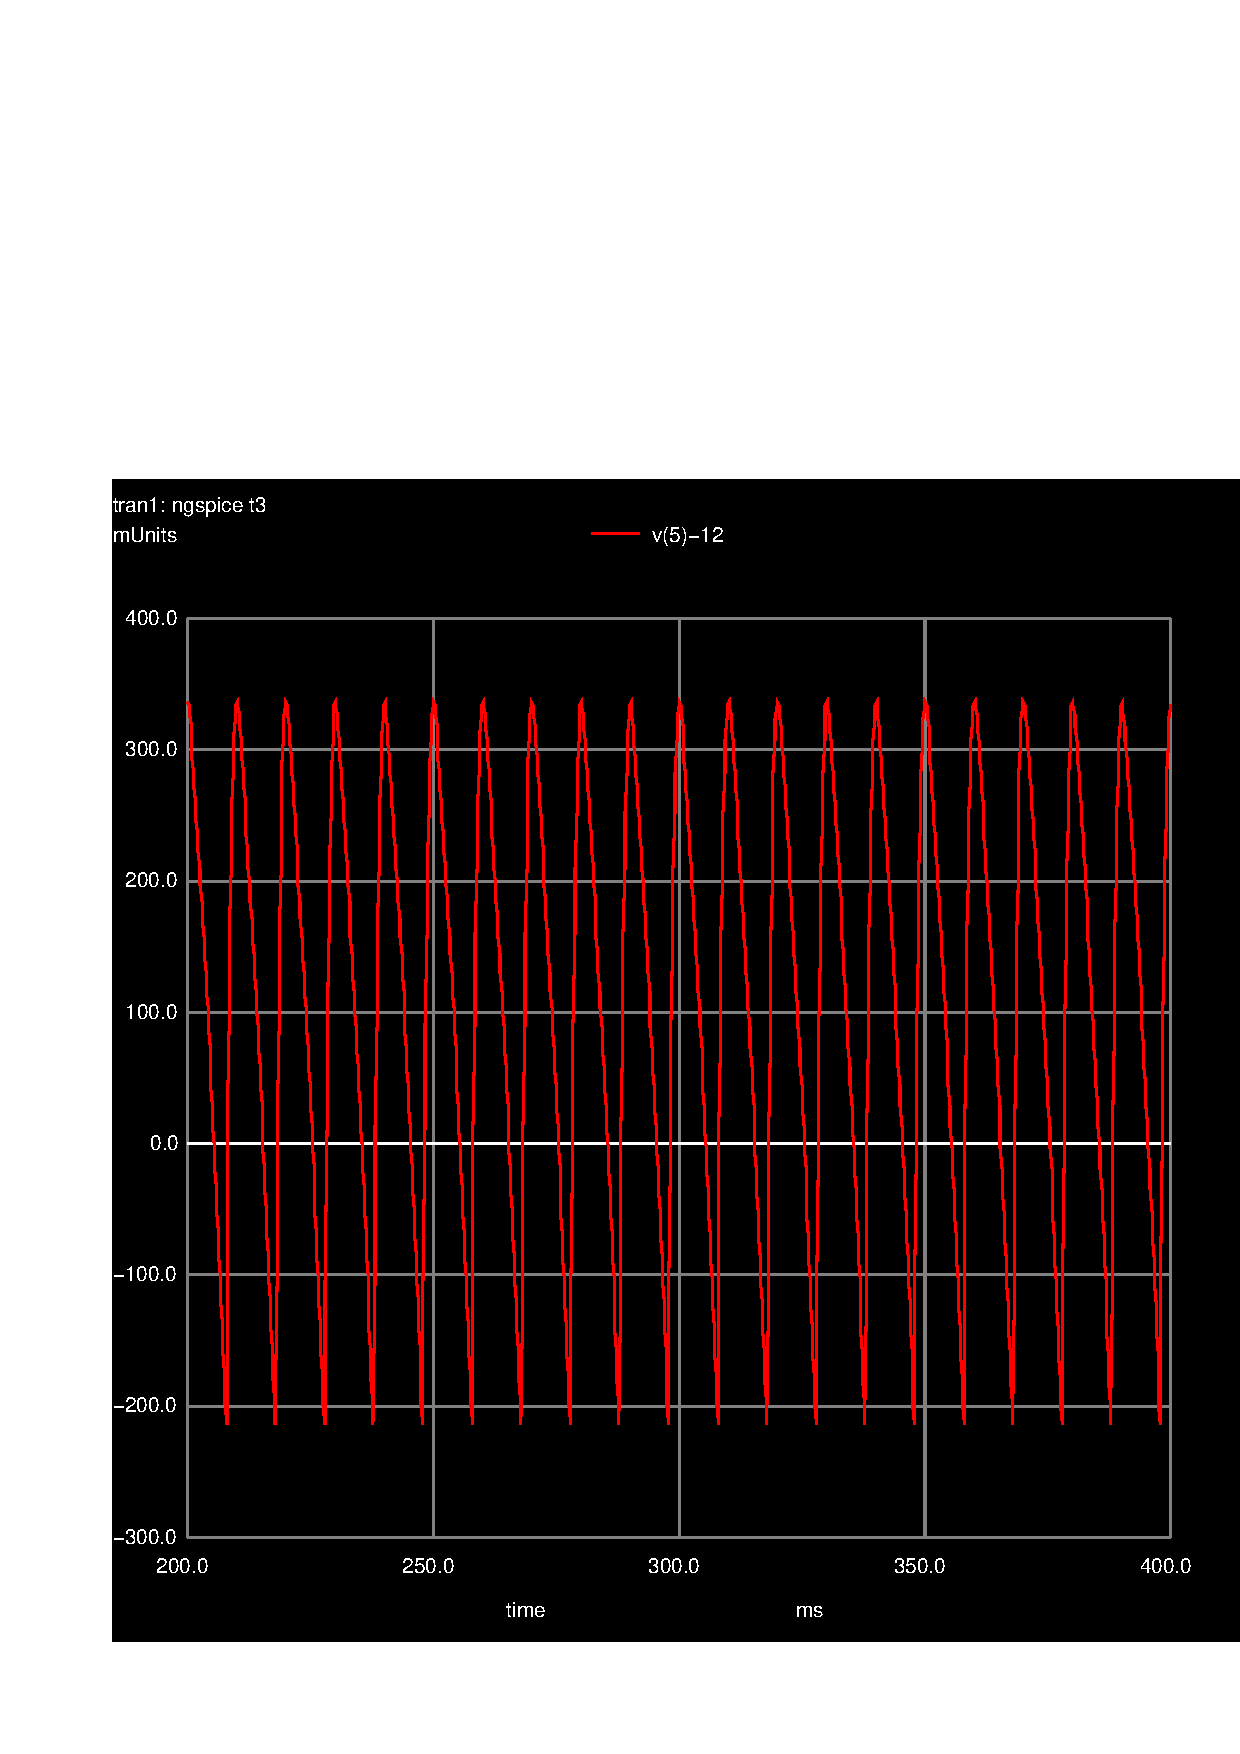
\includegraphics[width=0.4\linewidth]{../sim/dev.pdf}
    \centering
    \caption{$v_0-12$(Analysis left vs Simulation right)}
    \label{mag}
\end{figure}

\par It is clear that both plots are almost identical, which proves the success of the simulation. We can also conclude that the Envelope Detector and Voltage circuits designed by the group worked as expected and theorized when simulated.

